\chapter{Revisão bibliográfica}
Este capítulo aborda as teorias e conceitos que foram necessários para a realização da
pesquisa. Será elaborado uma revisão dos principais tópicos que explicam um melhor entendi-
mento sobre o amplo conceito de arquitetura de software e quais arquiteturas utilizaremos neste
trabalho.


\section{Arquitetura de micro serviços}
A Arquitetura de sistemas é um processo desafiador e crucial, principalmente em startups
que precisam lançar o produto o mais rápido possível. É de extrema importância também para
organizações que desejam melhorar, ou garantir, a eficiência, segurança e manutenção de seus
sistemas. Segundo \cite{Martin2017}, "a arquitetura é o conjunto de decisões que você queria ter
tomado logo no início de um projeto, mas, como todo mundo, não teve imaginação necessária".
Além disso, o crescimento do mercado, cria oportunidades para profissionais especializa-
dos nessa área. Com o crescimento do mercado, também as empresas buscam mais competitivi-
dade, lucratividade, com um software bem arquitetado, podemos garantir um custo mais baixo,
na implementação de novas funcionalidades, nos custos de Cloud e também de novos produtos.

Arquitetura de software é um conceito bem antigo, porém, nos últimos anos, houve
uma crescente demanda sobre a posição de Arquitetos de Solução nas empresas, muitas vezes
trabalhando como profissionais multidisciplinares, arquitetam, desenvolvem Designs System,
criam a documentação, e por muitas vezes, atuam também como líderes técnicos de times de
desenvolvimento.

Gigantes da tecnologia, que também são startups, muitas vezes compartilham suas
arquiteturas através da internet, para as pessoas terem conhecimento da complexidade do sistema
deles, como a imagem abaixo ilustra, a arquitetura de processamento de pagamento da Uber:
É um tema complexo e abrangente, discutido abertamente entre as pessoas técnicas e as
mais diversas corporações no mundo inteiro, além de ser necessário para todas as aplicações,
claramente, se a aplicação não tem um grande retorno financeiro ou uma grande complexidade,
não se tem a necessidade de ter um profissional especializado ou exclusivo para esse tema, porém,
é de extrema importância ter um profissional com experiência ou conhecimento técnico no time.
Obviamente, há diversos modelos de arquitetura desenvolvidos pela comunidade, ou
por grandes profissionais da computação em uso atualmente. Cada dia mais vem surgindo
novos modelos de arquitetura para satisfazer as necessidades de projetos. Para esse trabalho, por
exemplo, utilizaremos mais de um padrão arquitetural, a fim de abordar uma arquitetura ideal
para o projeto proposto.

É definido por \cite{Newman2015}, é uma abordagem que divide uma aplicação em
pequenos serviços independentes, cada um com uma única responsabilidade e modelado em
torno de um domínio de negócios. Esses serviços autônomos trabalham juntos e podem ser
desenvolvidos, implantados e escalados de maneira independente, o que facilita a modularidade,
melhorando a manutenção e o desenvolvimento do sistema.

\begin{figure}[!ht]
    \centering
    \caption{Arquitetura de micro-serviços}
    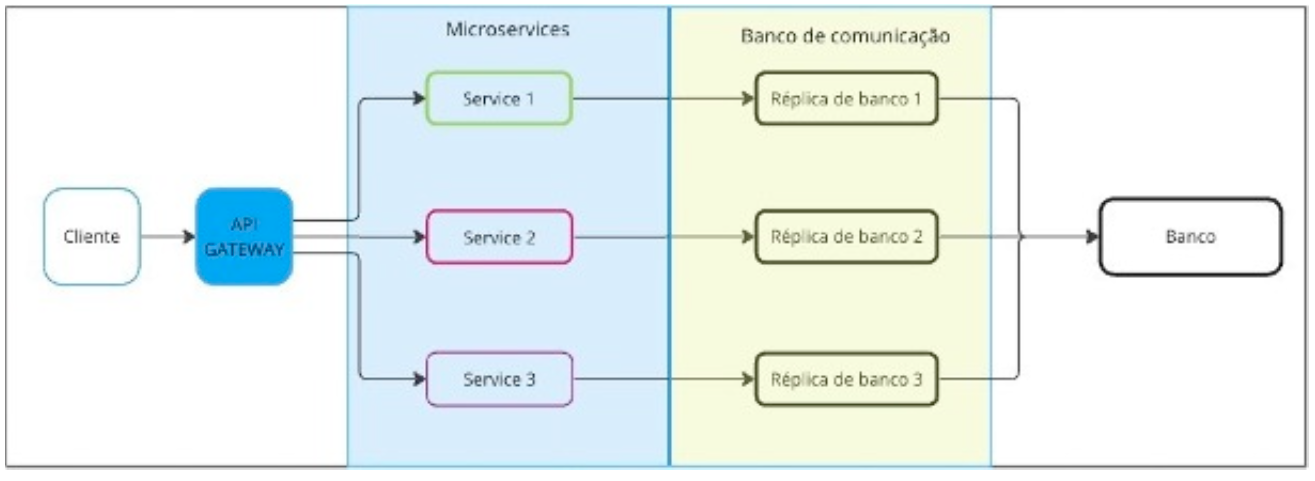
\includegraphics[scale=0.44]{assets/ms-arch}
    \label{fig:ms-arch}
    \tiny
    \sourcemedaddy
\end{figure}

Este modelo arquitetônico surgiu para solucionar desafios relacionados à escalabilidade,
eficiência, velocidade de desenvolvimento e acoplamento que são comumente encontrados em
arquiteturas monolíticas. Na arquitetura de micro serviços, cada serviço possui uma independên-
cia que garante a continuidade do funcionamento do sistema mesmo se um serviço individual
estiver indisponível \cite{Microsoft2023}.

A comunicação entre micro serviços é geralmente implementada através de APIs REST-
ful, que são baseadas em HTTP e aproveitam a infraestrutura da web \cite{LewisFowler}. No
entanto, em situações em que a latência é uma preocupação, outros protocolos de comunicação,
como o gRPC, podem ser usados.
Além disso, em operações que não exigem uma resposta
imediata, a comunicação pode ser assíncrona, com a utilização de sistemas de mensagens como
RabbitMQ ou Kafka \cite{Boner2019}.
Segundo a Microsoft, alguns dos benefícios sobre
essa arquitetura são:

\begin{itemize}
    \item \textbf{Agilidade:} ao ter um sistema quebrado em pequenos serviços, é mais ágil gerenciar correção de bugs, lançamento de recursos, além de poder reverter uma atualização se algo der errado;
    \item \textbf{Equipes pequenas e focadas:} um micro serviço deve ser pequeno o suficiente para apenas uma equipe mantê-lo, deixando a comunicação e desenvolvimento mais ágil, tendo em vista que equipes grandes tendem a ser menos produtivas, pois a comunicação é lenta e depende demais de gerenciamento;
    \item \textbf{Base de código pequena:} ao termos uma codebase, ou base de código, pequena, as dependências de código ficam menos emaranhadas, com um encapsulamento menor e menos dependências externas;
    \item \textbf{Mistura de tecnologia:} como os serviços são independentes, cada um pode ter uma linguagem de programação diferente, utilizando uma tecnologia que se adapta ao serviço melhor;
    \item \textbf{Isolamento de falhas:} se um micro serviço individual fica indisponível, ele não interrompe todo o aplicativo, desde que projetados para lidar com falhas, utilizando alguns padrões, como Circuit Breaker, ou se comunicando assincronamente;
    \item \textbf{Escalabilidade:} os serviços podem ser dimensionados independentemente, utilizando Kubernetes ou Service Fabric, por exemplo, você pode dimensionar subsistemas que exigem mais recursos;
    \item \textbf{Isolamento de dados:} é mais simples realizar atualizações de esquema, e apenas um único micro serviço é afetado, diferente de um monólito onde um todo é afetado.
\end{itemize}

Porém, temos também algumas desvantagens e/ou desafios ao implementar essa arquite-
tura, assim como:

\begin{itemize}
    \item \textbf{Complexidade:} para algumas aplicações, você implementa uma complexidade não necessária;
    \item \textbf{Desenvolvimento e testes:} as ferramentas existentes nem sempre são projetadas para funcionar com dependências de serviço. A refatoração entre limites de serviço pode ser difícil;
    \item \textbf{Falta de governança:} a abordagem descentralizada pode trazer problemas, principalmente se você tem diversas linguagens e uma gestão também descentralizada;
    \item \textbf{Integridade de dados:} como cada micro serviço é responsável pela sua própria persistência de dados, a consistência dos dados pode ser um dos desafios;
    \item \textbf{Gestão:} para desenvolver uma aplicação com grandes quantidades de serviços, deve-se ter uma cultura de DevOps madura, e os registros devem correlacionar várias chamadas de serviço para uma única operação de usuário.
\end{itemize}

Embora o uso de micro serviços ofereça muitos benefícios, também há desafios e desvan-
tagens, como a complexidade adicional para coordenação de serviços e a necessidade de uma
infraestrutura robusta para gerenciamento e monitoramento \cite{OReilly2018}.

Grandes empresas como a Netflix e a Amazon adotaram a arquitetura de micro serviços
para lidar com seus volumes massivos de transações e permitir a implantação contínua de
novos recursos \cite{BLOG2015}. No entanto, cada implementação tem suas
peculiaridades e, em alguns casos, como o da Amazon Prime Video, a migração para uma
arquitetura mais monolítica foi considerada mais benéfica \cite{Targett2023}.

\begin{figure}[!ht]
    \centering
    \caption{Arquitetura de micro-serviços AWS}
    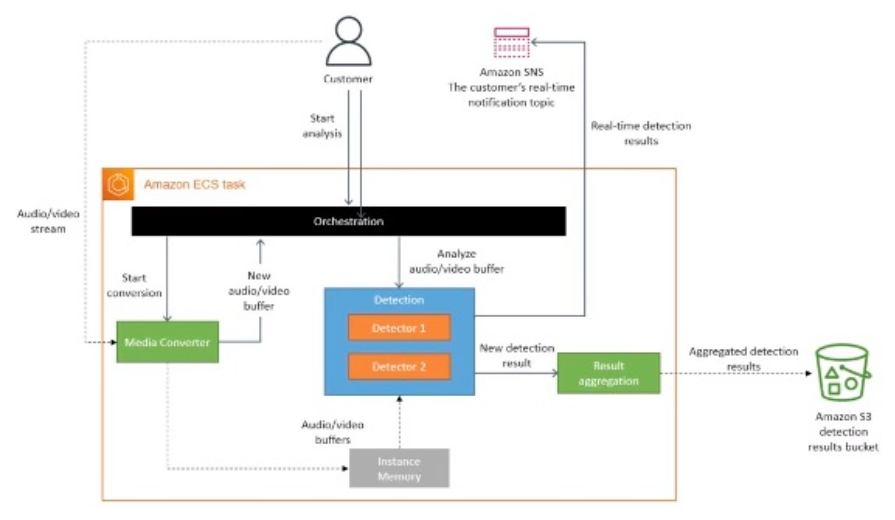
\includegraphics[scale=0.44]{assets/aws-ms}
    \label{fig:aws-ms}
    \tiny
    \sourcemedaddy
\end{figure}

Conforme imagem acima, a nova arquitetura, não foi migrada totalmente para monolito,
porém, conforme supracitado, já foi o suficiente para reduzir significativamente o custo de cloud;
por isso, deve-se tomar cuidado em abordagens como esta, pois, conforme ganha escala, o custo
fica mais caro.

Vale ressaltar que a adoção bem-sucedida de microserviços pode impactar significati-
vamente o desempenho e a escalabilidade dos sistemas \cite{Dragoni2017}. Portanto, é
crucial ponderar os benefícios e desafios antes de decidir por esta arquitetura.


\section{Arquitetura de mensageria}

A arquitetura de mensageria é uma das estratégias mais eficazes para gerenciar comuni-
cações entre serviços em um sistema distribuído, como os construídos com micro serviços.
Ela implementa comunicações assíncronas entre sistemas, geralmente recorrendo a tecnologias de
fila para garantir a entrega e o processamento de mensagens \cite{Boner2019}.

O paradigma de mensageria proporciona alta disponibilidade e resiliência, pois, mesmo que um serviço esteja temporariamente indisponível, as mensagens enviadas para ele serão armazenadas na fila até que o serviço esteja operacional novamente.
Essa característica é fundamental para sistemas de alta performance e pode minimizar o impacto de falhas em partes individuais do sistema.

Além disso, essa abordagem facilita a comunicação entre serviços escritos em diferentes linguagens de programação, uma vez que a interface de comunicação é estabelecida por meio da troca de mensagens, em vez de chamadas de método diretas.
Isso ajuda a alcançar uma verdadeira independência de serviço, que é um dos princípios fundamentais da arquitetura de micro serviços \cite{Newman2015}.

Entretanto, apesar de suas vantagens, a arquitetura de mensageria também apresenta desafios.
Um deles é a complexidade adicional na orquestração de mensagens e na gestão das filas.
Outro desafio é a dificuldade de implementar operações que exigem sincronia imediata, uma vez que a natureza assíncrona da arquitetura de mensageria pode levar a latências na comunicação \cite{Mota2022}.

Para lidar com esses desafios, algumas soluções de middleware de mensagens, como
RabbitMQ, ActiveMQ e Kafka, fornecem recursos avançados, como garantias de entrega, suporte
para padrões de mensagens complexos e mecanismos para lidar com mensagens em caso de
falha no processamento \cite{Kleppmann2017}.

Portanto, ao projetar uma arquitetura de micro serviços, a arquitetura de mensageria é uma
estratégia importante a ser considerada.
Ela fornece uma maneira de lidar com as complexidades da comunicação entre serviços, oferecendo um alto nível de desacoplamento, escalabilidade e resiliência.

Essa arquitetura é utilizada também com webhooks, e arquitetura também orientada a
eventos, quando sistemas precisam abrir uma comunicação bidirecional, como por exemplo:
temos uma criação de um Lead em um CRM e ele precisa me retornar e esperamos o retorno, logo, aguardamos o evento para uma trativa, podemos ter uma comunicação bidirecional.

Segundo \cite{LewisFowler}, algumas vantagens de utilizar mensageria são:

\begin{itemize}
    \item \textbf{Assincronismo:} a aplicação produtora da mensagem não precisa se preocupar com a aplicação consumidora estar ativa, pois o Message Broker, API Gateway ou a fila se responsabiliza em entregar quando a aplicação fica ativa novamente;
    \item \textbf{Acoplamento:} baixo acoplamento na integração entre sistemas, deixando-a assíncrona;
    \item \textbf{Múltiplas linguagens:} é possível integrar sistemas com diferentes linguagens, utilizando-as em suas especialidades.
\end{itemize}

\textbf{Desvantagens de utilizar esse modelo arquitetural:}

\begin{itemize}
    \item \textbf{Complexidade:} por ter uma certa distribuição e poder ter múltiplas linguagens, pode haver uma complexidade no desenvolvimento e manutenção do sistema;
    \item \textbf{Sincronismo:} não é adequado para cenários que exigem sincronismo entre as aplicações.
\end{itemize}

\begin{figure}[!ht]
    \centering
    \caption{Comunicação de mensageria}
    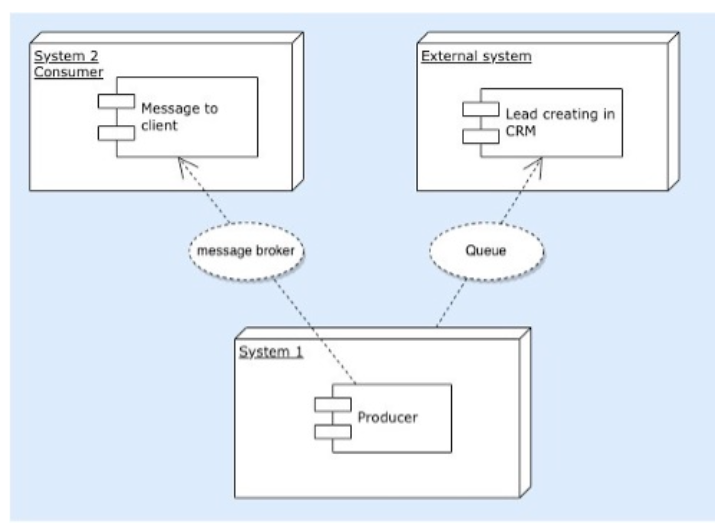
\includegraphics[scale=0.44]{assets/message-communication}
    \label{fig:message-communication}
    \tiny
    \sourcemedaddy
\end{figure}

\section{Arquitetura C4 model}
O modelo C4 é uma abordagem inovadora para a visualização da arquitetura de software.
Como mencionado anteriormente, ele foi criado por Simon Brown entre 2006 e 2011, com
o objetivo de superar as falhas na documentação e comunicação da arquitetura de software \cite{Brown2020}.

A arquitetura C4 model, ou apenas C4, consiste em uma forma ágil, com apelo téc-
nico para documentação da arquitetura de software e da parte técnica do sistema.
Segundo \cite{Santana2021} ela tem como premissa evitar dois principais cenários:

\begin{itemize}
    \item \textbf{Documentação de arquiteturas complexas:} documentações que demoram muito tempo para serem desenvolvidas ou que são difíceis de atualizar, com o tempo se tornam inutilizáveis ou obsoletas;
    \item \textbf{Documentações com poucas informações:} documentações pouco descritivas, com informações vagas ou falhas, também se tornam inutilizáveis.
\end{itemize}

O modelo C4 é baseado em quatro níveis de abstração, cada um dos quais visa um
público diferente e oferece um nível de detalhamento diferente. Isso torna o modelo C4 uma
ferramenta eficaz para a comunicação com diferentes partes interessadas, desde os não técnicos até os desenvolvedores de software \cite{Santana2021}.

O primeiro nível, o diagrama de contexto, proporciona uma visão de alto nível do sistema
em seu ambiente e é útil para comunicar a visão geral do sistema para todas as partes interessadas,
incluindo as não técnicas.
Este diagrama ilustra como o sistema interage com outros sistemas e usuários \cite{Brown2020}.

\begin{figure}[!ht]
    \centering
    \caption{Contexto C4 Model}
    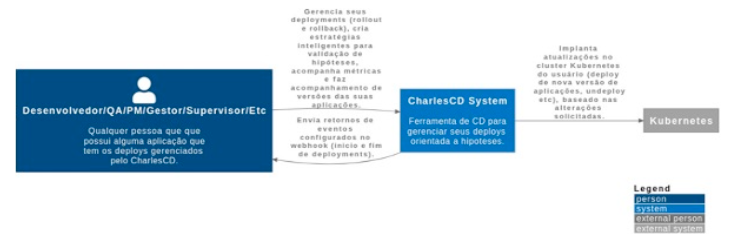
\includegraphics[scale=0.44]{assets/c4-context}
    \label{fig:c4-context}
    \tiny
    \sourcemedaddy
\end{figure}

O segundo nível, o diagrama de contêiner, é voltado para os desenvolvedores e outros
profissionais técnicos e mostra os principais componentes de alto nível do sistema, como bancos
de dados, servidores web, serviços de back-end e front-ends da web ou móveis, bem como suas
interações \cite{Brown2020}.

\begin{figure}[!ht]
    \centering
    \caption{Containers C4 Model}
    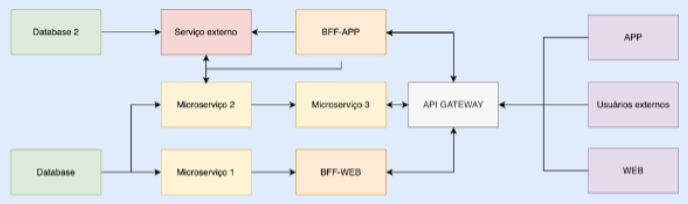
\includegraphics[scale=0.44]{assets/c4-containers}
    \label{fig:c4-containers}
    \tiny
    \sourcemedaddy
\end{figure}

O terceiro nível, o diagrama de componente, detalha ainda mais a estrutura interna de
cada contêiner, mostrando os diferentes componentes de software dentro de cada contêiner e
como eles interagem.
Este diagrama é útil para os desenvolvedores que trabalham no sistema \cite{Brown2020}.

\begin{figure}[!ht]
    \centering
    \caption{Componentes C4 Model}
    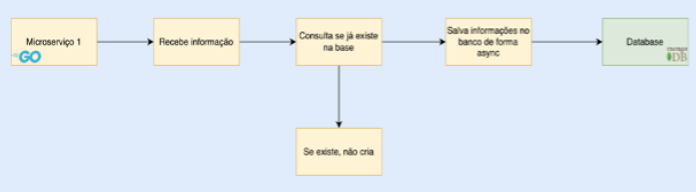
\includegraphics[scale=0.44]{assets/c4-components}
    \label{fig:c4-components}
    \tiny
    \sourcemedaddy
\end{figure}

Finalmente, o quarto nível, o diagrama de código, fornece uma visão detalhada de
algumas partes do código que são críticas para entender a implementação de determinados
componentes.
Este é o nível mais detalhado e é normalmente utilizado apenas quando necessário, devido à complexidade e ao esforço necessário para mantê-lo atualizado \cite{Brown2020}.

O modelo C4 é uma abordagem eficaz para documentar a arquitetura de software, pois
ajuda a comunicar a visão de alto nível e os detalhes técnicos de um sistema para diferentes
públicos.
No entanto, como qualquer ferramenta, ela deve ser usada adequadamente para ser
eficaz.
Isso significa que os diagramas devem ser mantidos atualizados à medida que o sistema
evolui e que o nível de detalhe deve ser adequado ao público-alvo \cite{Santana2021}.

\section{Node.JS/NestJS}

Node.js é um ambiente de tempo de execução de código aberto que permite a execução de
JavaScript no lado do servidor. Introduzido em 2009, o Node.js revolucionou o desenvolvimento
web ao permitir que os desenvolvedores criem aplicativos escaláveis e de alto desempenho
usando JavaScript tanto no cliente quanto no servidor.

De acordo com \cite{Silva2018}, o Node.js é construído com base
no mecanismo de JavaScript V8 do Google Chrome, o que o torna extremamente eficiente e
rápido. Ele usa um modelo de E/S não bloqueante, o que significa que é capaz de lidar com várias
solicitações simultaneamente, tornando-o ideal para aplicativos em tempo real, APIs RESTful e
outras aplicações de alto desempenho.

Nest.js, por sua vez, é um framework para Node.js construído com base no TypeScript.
Conforme mencionado por \cite{Tavares2020}, o Nest.js oferece uma arquitetura escalável e
modular que ajuda os desenvolvedores a criar aplicativos robustos e bem estruturados.
Ele usa conceitos familiares de outros frameworks populares, como Angular, tornando-o fácil de aprender
e usar para aqueles familiarizados com essas tecnologias.

De acordo com \cite{Johnson2020}, o Nest.js também enfatiza o uso de injeção de depen-
dência, o que facilita a criação de aplicativos altamente testáveis e extensíveis. Ele fornece um
sistema de módulos que ajuda a organizar e reutilizar o código de maneira eficiente, permitindo o
desenvolvimento de aplicativos complexos de forma mais gerenciável. Um aspecto importante do
Node.js e do Nest.js é o seu rico ecossistema de pacotes e bibliotecas. De acordo com (SANTOS,
2019), a comunidade em torno do Node.js contribuiu com uma ampla gama de módulos que
podem ser facilmente integrados aos projetos, facilitando o desenvolvimento de funcionalidades
avançadas.

\section{Typescript}

TypeScript é uma linguagem de programação de código aberto desenvolvida pela Micro-
soft que estende o JavaScript adicionando recursos de tipagem estática. Lançado em 2012, o
TypeScript foi projetado para melhorar o desenvolvimento de aplicativos JavaScript em larga
escala, fornecendo uma maneira de adicionar tipos aos objetos, variáveis e funções.

Segundo \cite{Farinha2018}, o TypeScript é baseado no ECMAScript
(padrão que define a linguagem JavaScript) e adiciona recursos como interfaces, classes, enu-
merações e suporte a tipos genéricos. Isso permite que os desenvolvedores escrevam código
mais robusto e seguro, identificando erros de digitação, chamadas de função incorretas e outros
problemas em tempo de compilação, antes mesmo de executar o código.

De acordo com \cite{Smith2019}, uma das principais vantagens do TypeScript é que ele
fornece um sistema de tipos opcional. Isso significa que os desenvolvedores podem escolher se
desejam adicionar tipos a seus códigos ou não. Quando os tipos são usados, o TypeScript pode
fornecer recursos avançados, como autocompletar, verificação estática de tipos e refatoração de
código.

Outro aspecto importante do TypeScript é sua compatibilidade com JavaScript existente.
De acordo com \cite{Johnson2020}, os desenvolvedores podem começar a adicionar gradualmente
o TypeScript a projetos JavaScript existentes, permitindo uma transição suave para a nova
linguagem. Além disso, o TypeScript é compilado para JavaScript padrão, o que significa que
pode ser executado em qualquer navegador ou ambiente que suporte JavaScript.

Segundo \cite{Oliveira2017}, o ecossistema do TypeScript também é robusto, com
suporte para várias bibliotecas e estruturas populares, como Angular, React e Node.js. Isso
permite que os desenvolvedores aproveitem os recursos do TypeScript ao trabalhar com essas
tecnologias.

Em resumo, o TypeScript é uma linguagem de programação que estende o JavaScript,
adicionando recursos de tipagem estática. Ele oferece benefícios como verificação de tipos em
tempo de compilação, autocompletar e compatibilidade com JavaScript existente. Ao adicionar
gradualmente o TypeScript a projetos JavaScript, os desenvolvedores podem melhorar a qualidade
e a segurança de seus códigos.


\section{GIT/GITHUB}
Git é um sistema de controle de versão distribuído amplamente utilizado no desenvolvi-
mento de software. Desenvolvido por Linus Torvalds em 2005, o Git oferece recursos poderosos
para o gerenciamento eficiente do código-fonte, rastreamento de alterações e colaboração em
projetos de programação.

Segundo \cite{Chacon2014}, o Git é conhecido por sua velocidade e efici-
ência, permitindo que os desenvolvedores trabalhem em projetos de qualquer tamanho com
facilidade. Ele utiliza um modelo distribuído, o que significa que cada desenvolvedor possui
uma cópia completa do repositório, incluindo todo o histórico de alterações. Isso permite que os
desenvolvedores trabalhem offline e sincronizem as alterações posteriormente.

Além disso, o Git usa um sistema de ramificação flexível.
De acordo com \cite{Loeliger2012}, os desenvolvedores podem criar ramificações (branches) independentes para desenvolver
recursos ou corrigir problemas sem interferir no trabalho principal.
Essas ramificações podem
ser mescladas (merged) de volta ao ramo principal quando estiverem prontas.
O GitHub, por sua vez, é uma plataforma de hospedagem baseada na web que utiliza o Git
para controle de versões.
Conforme apontado por \cite{Dabbish2012}, o GitHub oferece uma
interface amigável e recursos adicionais que facilitam a colaboração e o compartilhamento de
código entre desenvolvedores.
Ele permite que os desenvolvedores publiquem seus repositórios,
controlem as versões, gerenciem problemas e solicitações de alteração (pull requests) de forma
centralizada.

Segundo \cite{Chacon2016}, o GitHub também oferece recursos sociais, como
seguir outros desenvolvedores, contribuir para projetos de código aberto e revisar o código de
outras pessoas.
Essas funcionalidades promovem a colaboração e a comunidade em torno do
desenvolvimento de software.

O Git e o GitHub são amplamente utilizados na indústria de desenvolvimento de software
e são considerados essenciais para a maioria dos projetos. Eles permitem o controle eficiente
de versões, a colaboração em equipe e a criação de um histórico completo de alterações em um
projeto.

\section{PostgreSQL}

O PostgreSQL é um sistema de gerenciamento de banco de dados relacional de có-
digo aberto amplamente utilizado para armazenar e gerenciar dados em aplicativos modernos.
Introduzido em 1996, o PostgreSQL oferece uma abordagem robusta e escalável para o armaze-
namento de informações, permitindo que os desenvolvedores trabalhem com dados estruturados
de maneira eficiente.

De acordo com \cite{Momjian2001}, o PostgreSQL difere de outros bancos de dados
relacionais tradicionais por suportar extensibilidade e padrões SQL avançados. Isso significa que,
além dos tipos de dados tradicionais, o PostgreSQL permite a criação de novos tipos de dados,
índices e funções, tornando-o altamente flexível e personalizável para diversas necessidades de
aplicativos.

Uma das características mais importantes do PostgreSQL é sua conformidade com o
ACID (Atomicidade, Consistência, Isolamento e Durabilidade) e seu forte suporte a transações.
Conforme mencionado por \cite{stonebraker1986design}, o PostgreSQL permite a execução de
transações complexas com integridade de dados garantida, o que é essencial para aplicativos que
exigem confiabilidade em operações críticas.

Além disso, o PostgreSQL é conhecido por sua capacidade de escalar verticalmente
e horizontalmente. De acordo com \cite{stonebraker2010architecture}, ele pode ser configurado para
distribuir dados em várias máquinas por meio de replicação e particionamento, permitindo maior escalabilidade conforme a demanda aumenta. Isso é particularmente útil para aplicativos que
precisam lidar com grandes volumes de dados e requerem alta disponibilidade.

O PostgreSQL também oferece recursos avançados, como suporte a índices complexos,
consultas otimizadas e operações geoespaciais. De acordo com \cite{OBrien2016}, o PostgreSQL
permite consultas SQL avançadas e complexas, incluindo suporte a dados JSON, permitindo que
os desenvolvedores trabalhem com dados semiestruturados em paralelo com dados relacionais.
Como mencionado por \cite{pavlo2012comparison}, o ecossistema do PostgreSQL é amplamente
apoiado por uma comunidade ativa de desenvolvedores, além de oferecer diversas ferramentas e
integrações com outras tecnologias. O PostgreSQL também possui suporte em serviços gerencia-
dos na nuvem, como o Amazon RDS e o Google Cloud SQL, que facilitam sua implantação e
gerenciamento em ambientes de larga escala.

\section{Kafka}

O Apache Kafka é uma plataforma de streaming distribuída amplamente utilizada para processamento em tempo real e transmissão de dados em larga escala.
Introduzido em 2011, o Kafka foi projetado para lidar com altas taxas de dados, fornecendo um sistema de mensagens durável, tolerante a falhas e de alto desempenho.

Conforme descrito por \cite{Narkhede2018}, o Kafka adota uma
arquitetura distribuída e é capaz de lidar com grandes volumes de dados e fluxos de eventos. Ele
funciona em um modelo de publicação-subscrição, onde os produtores publicam mensagens em
tópicos, e os consumidores se inscrevem nesses tópicos para receber as mensagens em tempo
real. Essa abordagem torna o Kafka escalável e eficiente para fluxos de dados em tempo real.
Uma característica distintiva do Kafka é sua capacidade de armazenar e reter dados por
um período configurável. De acordo com \cite{Kreps2014}, o Kafka permite que as mensagens
sejam armazenadas em logs persistentes, permitindo a recuperação de dados históricos e a
realização de análises retroativas. Isso faz com que o Kafka seja uma escolha popular em casos
de uso como pipelines de dados, integração de sistemas e streaming de eventos.

Além disso, o Kafka oferece suporte a várias garantias de entrega de mensagens e opções
de particionamento. Conforme mencionado por \cite{sharma2017apache}, ele fornece mecanismos
de balanceamento de carga e replicação para garantir a confiabilidade e disponibilidade dos
dados. O particionamento permite que os dados sejam distribuídos em várias instâncias do Kafka,
permitindo o processamento paralelo e escalabilidade horizontal.

O ecossistema do Kafka também é rico em ferramentas e integrações. Segundo \cite{Garg2021}, existem bibliotecas e conectores disponíveis para uma variedade
de linguagens de programação e sistemas de armazenamento. Ademais, o Kafka pode ser
facilmente integrado a frameworks como o Apache Spark, permitindo o processamento de dados
em tempo real e análise de streaming.

\section{Monorepos}

Monorepos é uma abordagem de gerenciamento de código em que todo o código-fonte
de vários projetos relacionados é organizado em um único repositório de controle de versão. Essa
estrutura é amplamente adotada em projetos TypeScript para lidar com aplicativos complexos e
bibliotecas compartilhadas. Ao optar por um monorepo, os desenvolvedores podem aproveitar
várias vantagens, mas também podem enfrentar algumas desvantagens.

\subsection*{Vantagens dos monorepos em projetos TypeScript:}
\begin{itemize}
    \item \textbf{Compartilhamento de código}: Um dos principais benefícios dos monorepos é a capacidade de compartilhar código entre diferentes projetos. Com isso, é possível criar bibliotecas e componentes reutilizáveis em toda a base de código, o que resulta em maior eficiência de desenvolvimento e menos duplicação de código;

    \item \textbf{Gerenciamento simplificado de dependências}: Em um monorepo, todas as dependências são gerenciadas em um único local. Isso evita problemas de compatibilidade entre diferentes versões de dependências usadas em projetos separados, facilitando a atualização e manutenção do código;

    \item \textbf{Refatoração e colaboração simplificadas}: Com todo o código em um único repositório, a refatoração do código se torna mais fácil, pois as mudanças podem ser feitas em toda a base de código de uma só vez. Além disso, a colaboração entre equipes e desenvolvedores é aprimorada, pois todos estão trabalhando no mesmo repositório;

    \item \textbf{Versionamento consistente}: Em um monorepo, é possível ter um controle de versão consistente em toda a base de código. Isso significa que todos os projetos e bibliotecas compartilhadas avançam de versão juntos, o que facilita a rastreabilidade e a garantia de que todas as partes do sistema estejam em sincronia.
\end{itemize}

\subsection*{Desvantagens dos monorepos em projetos TypeScript:}
\begin{itemize}
    \item \textbf{Complexidade inicial}: Configurar um monorepo pode ser complexo, especialmente para equipes que estão migrando de uma estrutura de projeto tradicional. Requer um planejamento adequado para organizar a estrutura de pastas, configurar fluxos de construção e integração contínua, e definir as melhores práticas de desenvolvimento para colaboração efetiva;

    \item \textbf{Sobrecarga e tamanho do repositório}: À medida que o monorepo cresce e mais projetos são adicionados, o tamanho do repositório também aumenta. Isso pode levar a uma sobrecarga em termos de tempo de construção, consumo de espaço em disco e desempenho. Estratégias de otimização, como a utilização de ferramentas de construção incremental e empacotamento seletivo, são necessárias para lidar com esses desafios;

    \item \textbf{Acoplamento indesejado}: Em um monorepo, os projetos estão intimamente relacionados e compartilham o mesmo ciclo de versão. Isso pode resultar em um nível de acoplamento mais alto entre os componentes, o que pode dificultar a mudança independente de partes do sistema sem afetar outras partes;

    \item \textbf{Fluxo de trabalho compartilhado}: Embora a colaboração seja uma vantagem, também pode haver desafios no gerenciamento de um fluxo de trabalho compartilhado. Os conflitos de merge e a coordenação entre as equipes podem se tornar mais complexos em um monorepo.
\end{itemize}

\section{Docker}

O Docker é uma plataforma de virtualização de contêineres de código aberto que facilita
o desenvolvimento, implantação e execução de aplicativos em diferentes ambientes. Introduzido
em 2013, o Docker se tornou amplamente adotado na indústria de desenvolvimento de software
devido à sua capacidade de criar ambientes isolados e portáteis para a execução de aplicativos.

Conforme descrito por \cite{Boettiger2015}, o Docker utiliza a tecnologia de conteinerização para empacotar um aplicativo e todas as suas dependências em um contêiner leve e
autônomo. Esses contêineres são isolados uns dos outros, o que significa que cada aplicativo
pode ser executado de forma independente, sem interferir no sistema operacional ou em outros
contêineres.

\subsection*{Principais Vantagens do Docker}

\begin{itemize}
    \item \textbf{Portabilidade}: Segundo \cite{turner2019docker}, os containers Docker são executados da mesma maneira em qualquer ambiente que tenha o Docker instalado, seja em uma máquina local, em um ambiente de nuvem ou em um cluster de servidores. Isso simplifica o processo de implantação e evita problemas de inconsistência entre ambientes de desenvolvimento, teste e produção;

    \item \textbf{Escalabilidade}: De acordo com \cite{Muller2018}, o Docker permite que os aplicativos sejam facilmente dimensionados horizontalmente, adicionando ou removendo contêineres conforme necessário. Isso é especialmente útil para lidar com picos de carga de tráfego, pois os contêineres podem ser replicados para lidar com a demanda e, em seguida, reduzidos quando a carga diminuir;

    \item \textbf{Recursos avançados}: Além disso, o Docker oferece recursos avançados, como gerenciamento de redes, volumes para persistência de dados e integração com ferramentas de orquestração, como o Docker Swarm e o Kubernetes. Conforme mencionado por \cite{Matsumoto2017}, esses recursos permitem uma gestão eficiente de infraestrutura e facilitam a criação de ambientes de desenvolvimento e implantação altamente automatizados.
\end{itemize}

\section*{Modelagem de Dados com UML}

A modelagem de dados é uma prática fundamental no desenvolvimento de software para
representar visualmente a estrutura e o relacionamento dos dados em um sistema. A UML é uma
linguagem de modelagem padrão amplamente utilizada na indústria de software para descrever,
visualizar, especificar e documentar os aspectos do sistema.

De acordo com \cite{rumbaugh2004unified}, a UML oferece um
conjunto de notações gráficas que permitem aos desenvolvedores criar diagramas claros e
compreensíveis para representar diferentes perspectivas do sistema, incluindo a modelagem de
dados. Os diagramas UML ajudam a capturar as entidades, relacionamentos e atributos dos dados
de forma visual e organizada.

Um dos diagramas mais comumente usados para a modelagem de dados com UML é o
Diagrama de Classes. Segundo \cite{Larman2004}, o Diagrama de Classes permite representar
as classes do sistema, seus atributos e métodos, bem como os relacionamentos entre as classes,
como associações, agregações e heranças. Ele fornece uma visão estruturada dos dados e suas
interações no sistema.

Além do Diagrama de Classes, outros diagramas UML podem ser usados para complementar a modelagem de dados. Por exemplo, o Diagrama de Entidade-Relacionamento é útil para
representar as entidades e seus relacionamentos em um sistema de banco de dados. O Diagrama
de Atividades pode ser usado para modelar o fluxo de processos e a manipulação de dados dentro
do sistema.

A modelagem de dados com UML traz várias vantagens. Primeiramente, a UML oferece
uma notação padronizada e amplamente conhecida, facilitando a comunicação entre os membros
da equipe de desenvolvimento e outras partes interessadas. Além disso, a modelagem de dados
com UML permite uma compreensão clara e visual dos requisitos do sistema, facilitando a
identificação de problemas e a validação do design antes da implementação.

É importante ressaltar que a UML é uma linguagem flexível e extensível, permitindo
adaptações e personalizações de acordo com as necessidades do projeto. Para mais, o uso eficaz
da UML na modelagem de dados requer conhecimento e prática adequados para garantir a
precisão e a eficácia dos diagramas criados.


\section*{Supabase e o Supabase Storage}

O Supabase é uma plataforma de desenvolvimento de código aberto que fornece serviços
de backend para aplicativos web e móveis. Ele é frequentemente descrito como uma alternativa ao
Firebase, oferecendo uma variedade de ferramentas e recursos que permitem aos desenvolvedores
construir rapidamente aplicações escaláveis e seguras. Entre os principais serviços do Supabase,
destaca-se o armazenamento de arquivos, que oferece uma solução robusta para gerenciamento
de dados e arquivos em nuvem.

Segundo \cite{Gregoire2021}, o Supabase Storage permite que os desenvolvedores armazenem
e acessem arquivos, como imagens, vídeos e documentos, de forma rápida e eficiente. A
plataforma oferece uma API intuitiva que facilita a realização de operações de upload e download,
além de possibilitar a configuração de regras de segurança para proteger os dados armazenados.

Uma das características mais notáveis do Supabase Storage é a sua escalabilidade. De
acordo com a documentação oficial do \cite{supabase2023documentation}, o sistema é projetado para crescer
junto com as necessidades do aplicativo, permitindo que os desenvolvedores armazenem grandes
volumes de dados sem comprometer a performance. Essa escalabilidade é especialmente valiosa
em cenários onde o tráfego de usuários pode aumentar repentinamente.

Além disso, o Supabase se integra perfeitamente com outras funcionalidades da plataforma, como autenticação e banco de dados em tempo real. Como observado por \cite{Miller2022}, essa integração oferece aos desenvolvedores uma experiência coesa, permitindo que gerenciem autenticações de usuários, façam consultas a dados em tempo real e armazenem arquivos em um único ambiente.

Outra vantagem significativa do Supabase Storage é sua abordagem de segurança. A
plataforma permite que os desenvolvedores implementem regras de acesso personalizadas,
garantindo que somente usuários autorizados possam acessar ou modificar determinados arquivos.
Conforme afirmado por \cite{ONeill2022}, isso é crucial para proteger informações sensíveis e
garantir a privacidade dos dados armazenados.

\section*{API Gateway}

O API Gateway é um componente essencial na arquitetura de microservices, atuando
como um ponto de entrada centralizado para todas as solicitações de API. Ele desempenha
um papel fundamental na simplificação e na gestão do tráfego de API, fornecendo recursos
avançados, como autenticação, autorização, monitoramento e balanceamento de carga. Segundo
\cite{w3c2023webapi}, "um API Gateway é responsável por receber todas as solicitações de API, executar
qualquer lógica de negócio necessária e direcionar as solicitações para os serviços apropriados".

Uma das principais vantagens do API Gateway é a sua capacidade de encapsular a
complexidade das diferentes APIs e serviços subjacentes. Como mencionado por \cite{Kong2023},
uma empresa líder em soluções de gerenciamento de API, o API Gateway "fornecerá um único
ponto de entrada para várias APIs, independentemente de como essas APIs são implementadas
internamente". Isso permite que os desenvolvedores consumam várias APIs através de uma única
interface, simplificando a integração e o desenvolvimento de aplicativos.

Além da simplificação, o API Gateway também desempenha um papel importante na
segurança das APIs. Ele atua como um ponto de controle para autenticação e autorização,
garantindo que apenas as solicitações legítimas sejam direcionadas aos serviços subjacentes.
Conforme destacado pela \cite{AWS2023}, "o API Gateway protege suas APIs de ataques maliciosos,
como injeção de SQL, ataques de negação de serviço, entre outros". Isso é especialmente
importante em ambientes distribuídos, onde várias APIs são expostas e a segurança é uma
preocupação constante.

Outro aspecto relevante do API Gateway é a capacidade de fornecer recursos de mo-
nitoramento e análise. Ele permite rastrear e registrar dados relacionados ao tráfego de API,
incluindo métricas de desempenho, erros e padrões de uso. Com base nesses dados, as equipes
de desenvolvimento e operações podem obter insights valiosos sobre o desempenho das APIs
e identificar possíveis gargalos ou problemas de latência. De acordo com \cite{APIS2023}, "o
API Gateway é um local centralizado onde todas as métricas de API podem ser coletadas e
analisadas".

Além das funcionalidades mencionadas, o API Gateway também pode fornecer recursos
de transformação e composição de dados. Ele permite modificar a estrutura ou formato dos
dados transmitidos entre as APIs e os consumidores, facilitando a integração entre sistemas com
diferentes formatos de dados. Essa capacidade de transformação é particularmente útil quando
se lida com a exposição de APIs legadas ou quando é necessário agrupar dados de várias fontes
em uma única resposta.

\section{Considerações Finais do Capítulo}

Os objetivos propostos neste trabalho serão alcançados por meio de uma abordagem integrada e focada nas tecnologias e práticas modernas.
A aplicação da arquitetura de micro serviços permite uma estrutura flexível e escalável, essencial para atender às necessidades dinâmicas do projeto.
Essa arquitetura não apenas facilita o desenvolvimento, mas também promeve uma melhor gestão de cada componente da aplicação, contribuindo para um sistema mais resiliente.

A modelagem C4 será fundamental para descrever visualmente a estrutura do sistema, possibilitando uma compreensão clara das interações entre os micro serviços.
Isso ajudará a identificar possíveis gargalos e a otimizar as comunicações entre as partes do sistema, alinhando-se diretamente ao objetivo de desenvolver uma aplicação bem estruturada.

Por fim, a exploração de técnicas e tecnologias modernas não apenas proporciona eficiência no desenvolvimento, mas também garantiu a adoção de melhores práticas, resultando em um protótipo que está em sintonia com as demandas atuais do mercado.
